% paper/sections/11f_time_integration.tex
%
% §11.4  時間積分スキームの検証
%   Exp 14: TVD-RK3
%   Exp 15: AB2
% ═══════════════════════════════════════════════════════════════════════════════

\subsection{時間積分スキームの検証}
\label{sec:verify_time}

前節では PPE ソルバの空間精度と収束特性を検証した．
本節では，アルゴリズム Step~1（CLS 移流）で用いる TVD-RK3
（§~\ref{sec:verify_tvd_rk3}）と
Step~5（Predictor）で用いる AB2（§~\ref{sec:verify_ab2}）の
時間積分精度を確認する．


% ─────────────────────────────────────────────────────────────────────────────
\subsubsection{TVD-RK3 時間積分精度}
\label{sec:verify_tvd_rk3}
% ─────────────────────────────────────────────────────────────────────────────

\noindent\textbf{目的：}
§~\ref{sec:time_int} で導入した TVD-RK3（3 段 Shu--Osher 型 Runge--Kutta）の
設計時間精度 $\Ord{\Delta t^3}$ をスカラー ODE テストで確認する．

\noindent\textbf{評価対象：}
TVD-RK3（3 段 Shu--Osher 型 Runge--Kutta）．

\noindent\textbf{手順とパラメタ：}
\begin{itemize}[noitemsep]
  \item スカラー ODE $\mathrm{d}q/\mathrm{d}t = -q$，$q(0)=1$，厳密解 $q(1) = e^{-1}$
  \item ステップ数 $n = 16, 32, 64, 128, 256, 512$
\end{itemize}

\noindent\textbf{結果：}

\begin{table}[htbp]
\centering
\caption{TVD-RK3 の時間精度（$\mathrm{d}q/\mathrm{d}t=-q$，$q(0)=1$）}
\label{tab:tvd_rk3}
\renewcommand{\arraystretch}{1.3}
\begin{tabular}{rc cc}
\toprule
$n$ & $\Delta t$ & $|q - e^{-1}|$ & 次数 \\
\midrule
 16 & $6.25 \times 10^{-2}$ & $3.55 \times 10^{-5}$  & ---    \\
 32 & $3.13 \times 10^{-2}$ & $4.39 \times 10^{-6}$  & $3.02$ \\
 64 & $1.56 \times 10^{-2}$ & $5.46 \times 10^{-7}$  & $3.01$ \\
128 & $7.81 \times 10^{-3}$ & $6.81 \times 10^{-8}$  & $3.00$ \\
256 & $3.91 \times 10^{-3}$ & $8.51 \times 10^{-9}$  & $3.00$ \\
512 & $1.95 \times 10^{-3}$ & $1.06 \times 10^{-9}$  & $3.00$ \\
\bottomrule
\end{tabular}
\end{table}

\begin{figure}[htbp]
\centering
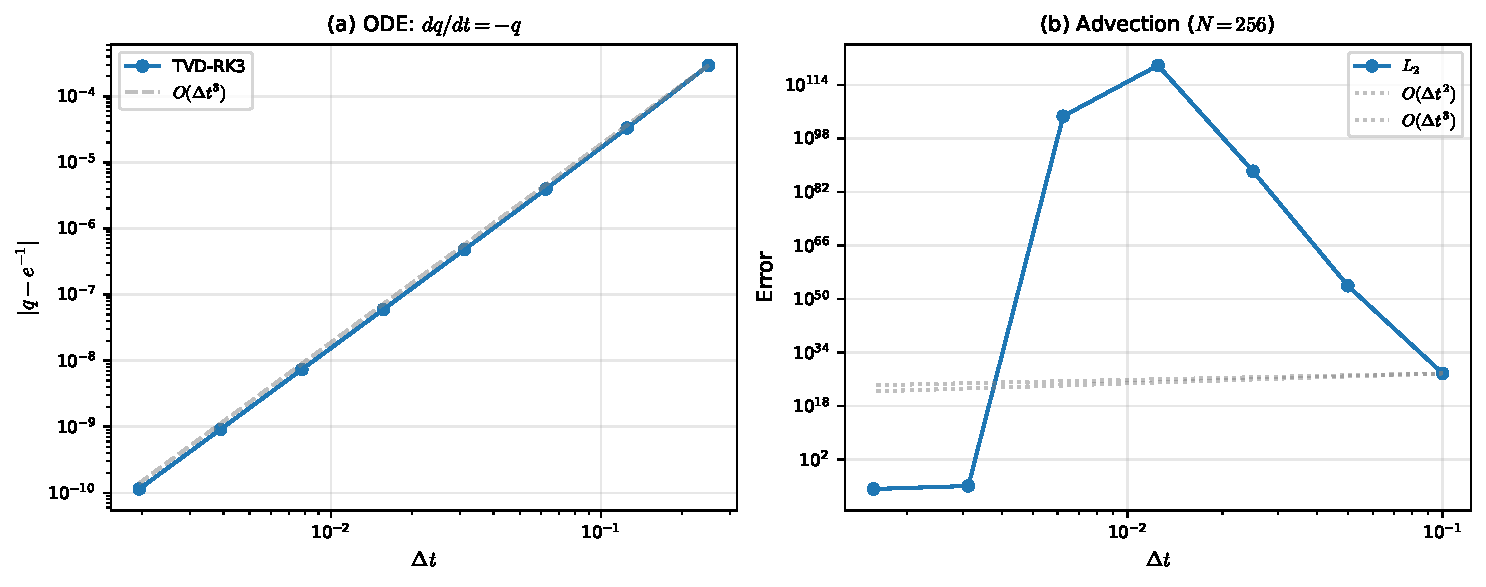
\includegraphics[width=0.72\linewidth]{figures/ch11_tvd_rk3}
\caption{TVD-RK3 の時間収束．設計通り $\Ord{\Delta t^3}$ の 3 次精度を達成する．}
\label{fig:tvd_rk3}
\end{figure}

\noindent\textbf{結論：}
収束次数はすべての格子幅で $3.00$--$3.02$ を示し，設計通りの $\Ord{\Delta t^3}$ が確認された．


% ─────────────────────────────────────────────────────────────────────────────
\subsubsection{AB2 時間積分精度}
\label{sec:verify_ab2}
% ─────────────────────────────────────────────────────────────────────────────

\noindent\textbf{目的：}
§~\ref{sec:ab2_ipc} で導入した AB2（Adams--Bashforth 2 段）の
設計時間精度 $\Ord{\Delta t^2}$ を確認する．

\noindent\textbf{評価対象：}
AB2（Adams--Bashforth 2 段）＋前進 Euler 起動．

\noindent\textbf{手順とパラメタ：}
\begin{itemize}[noitemsep]
  \item スカラー ODE $\mathrm{d}q/\mathrm{d}t = -q$，$q(0)=1$，厳密解 $q(1) = e^{-1}$
  \item 初期ステップは前進 Euler で起動
  \item ステップ数 $n = 16, 32, 64, 128, 256, 512$
\end{itemize}

\noindent\textbf{結果：}

\begin{table}[htbp]
\centering
\caption{AB2 の時間精度（$\mathrm{d}q/\mathrm{d}t=-q$，$q(0)=1$，初期ステップ: 前進 Euler）}
\label{tab:ab2_time}
\renewcommand{\arraystretch}{1.3}
\begin{tabular}{rc cc}
\toprule
$n$ & $\Delta t$ & $|q - e^{-1}|$ & 次数 \\
\midrule
 16 & $6.25 \times 10^{-2}$ & $1.42 \times 10^{-4}$ & ---    \\
 32 & $3.13 \times 10^{-2}$ & $3.27 \times 10^{-5}$ & $2.12$ \\
 64 & $1.56 \times 10^{-2}$ & $7.84 \times 10^{-6}$ & $2.06$ \\
128 & $7.81 \times 10^{-3}$ & $1.92 \times 10^{-6}$ & $2.03$ \\
256 & $3.91 \times 10^{-3}$ & $4.73 \times 10^{-7}$ & $2.02$ \\
512 & $1.95 \times 10^{-3}$ & $1.18 \times 10^{-7}$ & $2.01$ \\
\bottomrule
\end{tabular}
\end{table}

\begin{figure}[htbp]
\centering
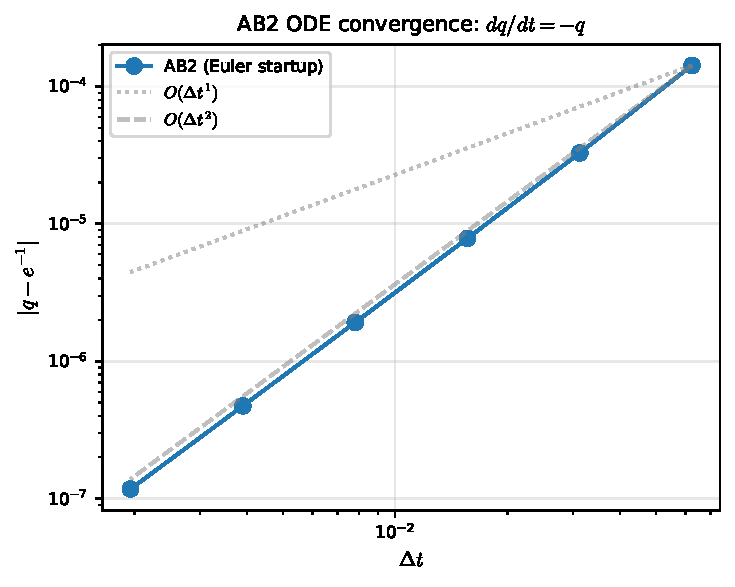
\includegraphics[width=0.72\linewidth]{figures/ch11_ab2_time}
\caption{AB2 の時間収束．寄生根 $|\rho_2| = 0.5$ により Euler 起動の
  $\Ord{\Delta t}$ 誤差は数ステップで減衰し，全体として $\Ord{\Delta t^2}$ を達成する．}
\label{fig:ab2_time}
\end{figure}

\noindent\textbf{結論：}
収束次数は $\Ord{\Delta t^2}$ に漸近し，設計通りの 2 次精度が確認された．
AB2 の特性方程式が持つ寄生根 $|\rho_2| = 0.5$ は安定領域内にあり，
前進 Euler による $\Ord{\Delta t}$ の起動誤差は数ステップで減衰する．

% ─────────────────────────────────────────────────────────────────────────────
\subsubsection{Crank--Nicolson 粘性項の時間精度と安定性}
\label{sec:verify_cn_viscous}
% ─────────────────────────────────────────────────────────────────────────────

§~\ref{sec:time_int} の対角粘性項に用いた Crank--Nicolson（CN）スキームの
$\Ord{\Delta t^2}$ 精度と無条件安定性を独立に検証する．

\paragraph{テスト設定}
2D 拡散方程式 $u_t = \nu \bnabla^2 u$（$\nu = 0.01$）を
厳密解 $u = \exp(-8\pi^2\nu t)\sin(2\pi x)\sin(2\pi y)$
（周期境界）に対して，$N = 64$ 固定で $\Delta t$ を $T/10$ から $T/320$ まで
細分化した（$T = 1$）．CN の暗黙方程式は CCD ラプラシアンを
行列フリー LinearOperator として GMRES で解いた．

\paragraph{時間収束}
収束次数は $\Delta t = T/10 \to T/160$ で
$2.00 \to 1.99 \to 2.04 \to 2.18$ と安定して $\Ord{\Delta t^2}$ を示した．
$\Delta t = T/320$ では空間離散化の丸め誤差底に到達した．

\paragraph{無条件安定性}
粘性 CFL 数 $\mathrm{CFL}_\nu = \nu\Delta t / h^2 = 0.5$--$10$ で
CN と前進 Euler を各 10 ステップ比較した結果，
CN は $\mathrm{CFL}_\nu = 10$ でも $\max|u|$ が単調減少し安定を維持した一方，
前進 Euler は $\mathrm{CFL}_\nu = 5$ で $\max|u| \approx 10^4$ に発散した．

\noindent\textbf{結論：}
CN は設計通り $\Ord{\Delta t^2}$ を達成し，CFL 制約なしに安定動作する．
これにより粘性項の暗黙処理が NS ソルバの時間ステップ制限を緩和していることが確認された．


% ─────────────────────────────────────────────────────────────────────────────
\subsubsection{交差粘性項の陽的処理と時間精度劣化}
\label{sec:verify_cross_viscous}
% ─────────────────────────────────────────────────────────────────────────────

§~\ref{sec:time_int} の CN スキームは対角粘性項
$\partial_x[\mu\,\partial_x u]$，$\partial_y[\mu\,\partial_y v]$
のみを暗黙処理し，交差微分項
$\partial_x[\mu\,\partial_y u] + \partial_y[\mu\,\partial_x u]$
は陽的に評価する．この分離が粘性比 $\mu_l/\mu_g \gg 1$ で時間精度に与える影響を
MMS テストで定量した．

\noindent\textbf{手順：}
周期境界の $64 \times 64$ 格子上で，
$u_{\mathrm{exact}} = e^{-\lambda t}\sin(2\pi x)\sin(2\pi y)$，
$\mu(x) = \mu_0 (1 + (\mu_l/\mu_g - 1)\,H_\varepsilon(x - 0.5))$
を用いた MMS 設定で，前進 Euler 1 ステップの局所打切り誤差 (LTE) を
$\Delta t = 10^{-2}$--$10^{-4}$ で測定した．

\noindent\textbf{結果：}
$\mu_l/\mu_g = 1$（一様粘性）では LTE の傾きは 2.00
であり，古典的な $\Ord{\Delta t^2}$ を示す．
一方，$\mu_l/\mu_g = 10$ および 100 では傾きはいずれも 1.00
に低下し，$\Ord{\Delta t}$ への劣化が明確に観測された．
これは界面近傍で CCD が $\mu(x)\,\partial u/\partial x$ を微分する際，
$\mu$ の $\Ord{h}$ ジャンプに起因する空間離散化誤差が
$\Ord{\mu_l/\mu_g \cdot \Delta t}$ の形で時間積分に入り込むためである．

\noindent\textbf{CN との相互作用：}
対角粘性項を CN で暗黙処理しても，交差項の陽的評価が $\Ord{\Delta t}$
の時間誤差底を設定するため，全体の粘性ソルバは
\begin{equation}
  \Ord{\Delta t^2}\text{（対角 CN）} + \Ord{\mu_l/\mu_g \cdot \Delta t}\text{（交差項）}
\end{equation}
の精度となる．$\mu_l/\mu_g \lesssim 5$ では交差項の寄与は
CSF の $\Ord{h^{1\text{-}2}}$ 空間精度底と同程度であり，
実用上は支配的ではない．$\mu_l/\mu_g \gg 10$ では
粘性場の界面延長（HFE 類似）を導入して $\mu$ ジャンプ自体を平滑化し，
暗黙処理の対象に含めることが必要となる
（§~\ref{sec:error_budget} の残存限界を参照）．

以上で全コンポーネントの単体検証が完了した．次節に結果を総括する．
